\documentclass[12pt]{article}
\title{Introduction to Boolean networks}
\author{Adam Streck \\
		Discrete Biomathematics, FU Berlin}
\usepackage{alltt}
\usepackage{a4wide}
\usepackage{pgf}
\usepackage{tikz}

%Environments used for description of DBM
\newenvironment{menum}{
\begin{enumerate}
  \setlength{\itemsep}{0pt}
  \setlength{\parskip}{0pt}
  \setlength{\parsep}{0pt}
}{\end{enumerate}}
\newenvironment{mitem}{
\begin{itemize}
  \setlength{\itemsep}{0pt}
  \setlength{\parskip}{0pt}
  \setlength{\parsep}{0pt}
}{\end{itemize}}

\begin{document}
\maketitle


To help with understanding of concepts of the formal modeling framework used in Esther we demonstrate basic notions on a very simple example of a regulatory network, depicted in Figure~\ref{ExampNet}. This network has two boolean components named $cA$ and $B$, each regulated by both itself and the other component. This a bit unconventional naming has been choosen to demonstrate variability of modeling language later in the Section~\ref{sec:modeling}.

The model is a boolean one, which means that there are only two activity levels for each component, roughly corresponding to the situations where its concentration is below threshold or above it. The threshold marks a concentration boundary whose crossing usually causes the component to change its regulatory effect. Boolean component therefore usually works as a switch.

\begin{figure}[b]
\centering
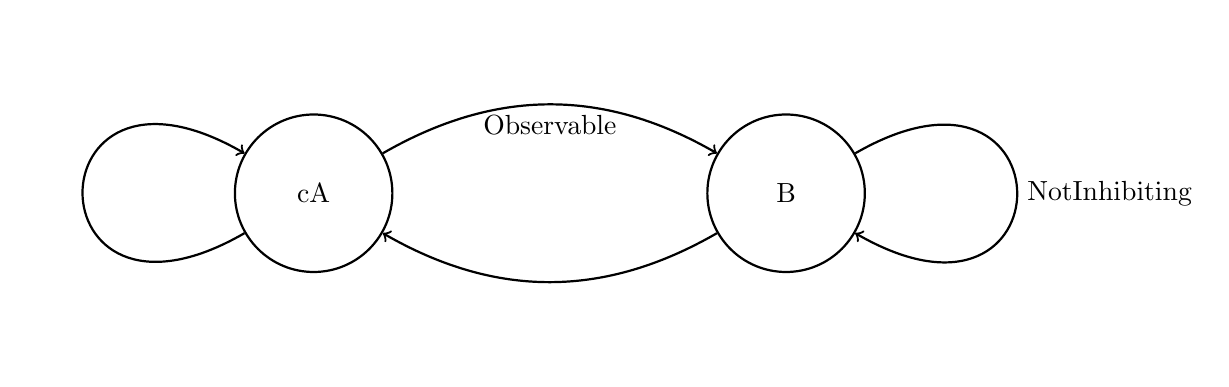
\begin{tikzpicture}
\node[draw, circle, thick, minimum size=20mm] (cA) at (0,0) {cA};
\node[draw, circle, thick, minimum size=20mm] (Y) at (6,0) {B};
\draw[->, thick] (cA) to [in=150,out=210,loop] (cA);
\draw[->, thick] (cA) to [bend left=30] node[below] {Observable} (Y);
\draw[->, thick] (Y) to [bend left=30] (cA);
\draw[->, thick] (Y) to [in=330,out=30,loop] node[right] {NotInhibiting} (Y);
\end{tikzpicture}
\caption{Simple example network with two components.}
\label{ExampNet}
\end{figure}

Components of such a network are usually well-know, conversely to their regulatory effects that are hard to obtain from biological measurements~\cite{Hecker09}. The Parsybone is designed to solve the task of determining those effects or at least to narrow the set of posibilities thus helping with further analysis. Possible regulatory effects of a component are given by the so-called \emph{logical parameters}. Each component has usually several logical parameters that specify towards which activity level the component inclines based on the current activity levels of its regulators e.g. a self-regulating component can stop its production when a certain concentration level is reached.

The user is required to specify the model as a set of components and their interactions. Having such a model, the Parsybone generates all possibile combinations of logical parameters for the model, creating a set of \emph{parametrizations}. This set is usually called \emph{parametrization space} and it can be viewed as a set of all behavioural possibilities for the model. As a second input, the Parsybone takes a specification of some behaviour the model must be able to reproduce. Parametrizations that do not allow such a behaviour are then removed from the set of possibilities.

Apart from basic boolean properties we also allow the model to be created using multiple extensions:
\begin{itemize}
\item Multi-valued components, allowing to change the effect of only a subset of its regulatory effects at a time.
\item Edge labels, bounding possible effects of the regulations.
\item Partial parametrizations, allowing to reduce the parametrization space before the analysis itself.
\item Basal values, specifying general case behaviour of components.
\end{itemize}

These extension allow for more precise model description than the basic boolean network formalism as presented above, but their explanation is beyond scope of this section. In case of furter interest please refer to~\cite{TechReport}.

\bibliographystyle{abbrv}
\bibliography{Manual}

\end{document}